% This file is part of The Cannon.
% Copyright 2017 David W. Hogg (NYU).

\documentclass[pdftex]{beamer}
\input{vc}
% 1.77778 is the ratio of 16 to 9
\setlength{\paperheight}{2.9in}
\setlength{\paperwidth}{1.77778\paperheight}
% 1.33333 is the ratio of 4 to 3
%\setlength{\paperheight}{3.2in}
%\setlength{\paperwidth}{1.33333\paperheight}
% textwidth
\setlength{\textwidth}{0.85\paperwidth}
% import the next thing *after* the papersize
\usepackage{amssymb,amsmath,mathrsfs}
\usecolortheme{default}

% this one is debatable
\renewcommand{\emph}[1]{\textbf{#1}}

%%% color commands
\newcommand{\whiteonblack}{%
  \colorlet{fg}{white}
  \colorlet{bg}{black}
  \setbeamercolor{normal_text}{fg=white,bg=black}
  \setbeamercolor{background canvas}{fg=white,bg=black}
  \setbeamercolor{alerted_text}{fg=yellow}
  \setbeamercolor{example_text}{fg=white}
  \setbeamercolor{structure}{fg=white}
  \setbeamercolor{palette_quaternary}{fg=white}
}
\newcommand{\blackonwhite}{%
  \colorlet{fg}{black}
  \colorlet{bg}{white}
  \setbeamercolor{normal_text}{fg=black,bg=white}
  \setbeamercolor{background canvas}{fg=black,bg=white}
  \setbeamercolor{alerted_text}{fg=blue}
  \setbeamercolor{example_text}{fg=black}
  \setbeamercolor{structure}{fg=black}
  \setbeamercolor{palette_quaternary}{fg=black}
}
\xdefinecolor{pink}{rgb}{1.0,0.9,0.9}

%%% size and shape commands
\newlength{\figurewidth}
\setlength{\figurewidth}{0.9\textwidth}
\newlength{\figureheight}
\setlength{\figureheight}{0.9\textheight}

%%% text commands
\newcommand{\project}[1]{\textsl{#1}}
  \newcommand{\an}{\project{Astrometry.net}}
  \newcommand{\euclid}{\project{Euclid}}
  \newcommand{\flickr}{\project{flickr}}
  \newcommand{\gaia}{\project{Gaia}}
  \newcommand{\galex}{\project{GALEX}}
  \newcommand{\kepler}{\project{Kepler}}
  \newcommand{\GALEX}{\galex}
  \newcommand{\hst}{\project{HST}}
  \newcommand{\hipparcos}{\project{Hipparcos}}
  \newcommand{\lsst}{\project{LSST}}
  \newcommand{\sdss}{\project{SDSS}}
  \newcommand{\sdssiii}{\project{SDSS-III}}
  \newcommand{\sdssiv}{\project{SDSS-IV}}
  \newcommand{\boss}{\project{BOSS}}
  \newcommand{\apogee}{\project{APOGEE}}
  \newcommand{\osss}{\project{OSSS}}
  \newcommand{\ska}{\project{SKA}}
  \newcommand{\vo}{\project{VO}}
  \newcommand{\rttd}{\project{Right Thing To Do}$^{\mbox{\scriptsize\sffamily{TM}}}$}
\newcommand{\foreign}[1]{\textit{#1}}
\newcommand{\latin}[1]{\foreign{#1}}
  \newcommand{\cf}{\latin{cf.}}
  \newcommand{\eg}{\latin{e.g.}}
  \newcommand{\etal}{\latin{et~al.}}
  \newcommand{\etc}{\latin{etc.}}
  \newcommand{\ie}{\latin{i.e.}}
  \newcommand{\vs}{\latin{vs.}}

%%% math-mode commands
\newcommand{\unit}[1]{\mathrm{#1}}
  \newcommand{\rad}{\unit{rad}}
  \newcommand{\s}{\unit{s}}
  \newcommand{\yr}{\unit{yr}}
  \newcommand{\km}{\unit{km}}
  \newcommand{\kmps}{\km\,\s^{-1}}
\newcommand{\mmatrix}[1]{\boldsymbol{#1}}
\newcommand{\tv}[1]{\boldsymbol{#1}}
\newcommand{\dd}{\mathrm{d}}
\newcommand{\given}{\,|\,}
 % hogg standard colors

\newcommand{\credits}{{\footnotesize (Ness, Hogg, \etal)}}
\newcommand{\teff}{T_{\mathrm{eff}}}
\newcommand{\logg}{\log g}
\newcommand{\feh}{[\mathrm{Fe / H}]}
\newcommand{\alphafe}{[\mathrm{\alpha / Fe}]}

\title{The most precise measurements\\ of red-giant stars}
\author[David W. Hogg (NYU)]{\textbf{David W. Hogg} \\
  \textsl{\footnotesize Center for Cosmology and Particle Physics, Dept.~Physics, NYU} \\
  \textsl{\footnotesize Center for Data Science, NYU} \\
  \textsl{\footnotesize Max-Planck-Insitut f\"ur Astronomie, Heidelberg} \\
  \textsl{\footnotesize Flatiron Institute, Simons Foundation, New York City}}
\date{AIP / Wempe Award Ceremony / 2017 July 05}

\newcommand{\conclusions}{%
\begin{frame}
  \frametitle{conclusions}
  \begin{itemize}
  \item \emph{Data-driven models are delivering the most precise measurements
    of stellar parameters}, better than any physics-driven models.
    \begin{itemize}
    \item \tc\ for stellar spectra
    \item hierarchical models for photometry
    \end{itemize}
  \item (Everything public and open-source.)
  \item \emph{Melissa~Ness}~(MPIA), \emph{Andy~Casey}~(Cambridge), \emph{Anna~Y.~Q.~Ho}~(Caltech), \emph{Lauren Anderson}~(Flatiron), Boris Leistedt (NYU), Keith Hawkins (Columbia), Hans-Walter~Rix~(MPIA)
  \end{itemize}
\end{frame}}

\begin{document}\sloppy\sloppypar\raggedright\raggedbottom

\begin{frame}
  \titlepage
\end{frame}

\conclusions

\begin{frame}
  \frametitle{Alice Quillen}
  \begin{itemize}
  \item spiral and bar structure in disks
  \item heating and thickness of the disk
  \item radial migration
  \item disk modes and response to interactions
  \item (also: exoplanet dynamics)
  \end{itemize}
\end{frame}

\begin{frame}
  \frametitle{How do we measure these?}
  \begin{itemize}
  \item deep imaging
  \item astrometry
  \item infrared spectroscopy
  \item extremely precise models of stars
    \begin{itemize}
    \item (especially red-giant stars)
    \item distances, velocities; full phase-space vectors
    \item chemical tags
    \item ages
    \end{itemize}
  \end{itemize}
\end{frame}

\begin{frame}
  \frametitle{tools}
  \begin{itemize}
  \item This talk will be about \emph{tools}.
  \end{itemize}
\end{frame}

\begin{frame}
  \frametitle{accuracy and precision}
  \begin{itemize}
  \item The goal of physical models of stars is \emph{accuracy}
  \item There are many stellar properties that will not be known accurately in my lifetime.
    \begin{itemize}
    \item \eg, chemical abundances
    \item Is this controversial? How could we verify? Sample return?
    \end{itemize}
  \item Many scientific objectives require only \emph{precision} and \emph{consistency}.
    \begin{itemize}
    \item these are the goals of data-driven models
    \end{itemize}
  \end{itemize}
\end{frame}

\begin{frame}
  \frametitle{physics-driven models (my usage)}
  \begin{itemize}
  \item put in everything you know
    \begin{itemize}
    \item gravity, atomic and molecular transitions, radiation
    \end{itemize}
  \item make approximations to make things computable
    \begin{itemize}
    \item ``sub-grid'' models, mixing length, etc
    \end{itemize}
  \end{itemize}
\end{frame}

\begin{frame}
  \frametitle{machine learning}
  \begin{itemize}
  \item the most extreme of data-driven models
  \item ``the data \emph{is} the model''
    \begin{itemize}
    \item none of your knowledge is relevant
    \end{itemize}
  \item learn (fit) an exceedingly flexible model
    \begin{itemize}
    \item explain or cluster the data
    \item transformation from data to ``labels''
    \end{itemize}
  \item concept of non-parametrics
  \item concept of train, validate, and test
  \item many packages and implementations
    \begin{itemize}
    \item (and outrageous successes)
    \end{itemize}
  \end{itemize}
\end{frame}

\begin{frame}
  \frametitle{when does (vanilla) machine learning help you?}
  \begin{itemize}
  \item train \& test situation
  \item training data are statistically identical to the test data
    \begin{itemize}
    \item same noise amplitude
    \item same distance or redshift distribution
    \item same luminosities, metallicities, \ldots
    \item \emph{never true!}
    \end{itemize}
  \item training data have accurate and precise labels
  \item therefore, we \emph{can't use vanilla machine learning!}
    \begin{itemize}
    \item (physicists rarely can)
    \end{itemize}
  \end{itemize}
\end{frame}

\begin{frame}
  \frametitle{data-driven models (my usage)}
  \begin{itemize}
  \item make use of things you \emph{strongly believe}
    \begin{itemize}
    \item noise model \& instrument resolution
    \item causal structure (shared parameters)
    \end{itemize}
  \item capitalize on huge amounts of data
  \item exceedingly flexible model
  \item concept of train, validate, and test
  \item every situation will be \emph{bespoke}
  \end{itemize}
\end{frame}

\begin{frame}
  \frametitle{data-driven models}
  \begin{itemize}
  \item \tc
  \item hierarchical color-magnitude models
  \end{itemize}
\end{frame}

\begin{frame}
  \frametitle{Annie Jump Cannon}
  \begin{itemize}
  \item O B A F G K M
    \begin{itemize}
    \item temperature sequence!
    \item alphabetical order is hydrogen-line-strength order
    \end{itemize}
  \item Cannon understood the temperature sequence of stars without the benefit of physical models
    \begin{itemize}
    \item data-driven non-linear dimensionality reduction
    \item ``manifold learning''
    \item (using a huge amount of prior knowledge)
    \end{itemize}
  \item namesake of \tc
  \end{itemize}
\end{frame}

\begin{frame}
  \frametitle{\tc}
  \begin{itemize}
  \item a few of your stars have good labels (from somewhere)
  \item can you use this to label the other stars?
  \item why would you want to do this?
    \begin{itemize}
    \item<2> you don't have good models at your wavelengths?
    \item<2> you want two surveys to be on the same ``system''?
    \item<2> you have some stars at high SNR, some at low SNR?
    \item<2> you spent human time on some stars but can't on all?
    \end{itemize}
  \end{itemize}
\end{frame}

\begin{frame}
  \frametitle{chemodynamics or Galactic archaeology}
  \begin{itemize}
  \item stars populate orbits in the Milky Way
    \begin{itemize}
    \item (nearly) invariant ``actions''
    \item (or chaotic equivalents)
    \end{itemize}
  \item stars are formed from particular gas clouds
    \begin{itemize}
    \item (nearly) invariant surface abundances
    \item other invariants (birthday, etc)
    \end{itemize}
  \item the combined action-chemical space will be far more
    informative than either taken independently
  \end{itemize}
\end{frame}

\begin{frame}
  \frametitle{chemodynamics}
  \begin{itemize}
  \item top priority for many projects
    \begin{itemize}
    \item \project{\acronym{RAVE}}
    \item \gaia
    \item \project{Gaia-\acronym{ESO}}
      \&  \project{\acronym{GALAH}}
      \&  \project{\acronym{4MOST}}
      \&  \ldots
    \item \apogee (part of \sdssiii\ and \sdssiv)
    \end{itemize}
  \item terrifying inconsistencies in current approaches
    \begin{itemize}
    \item models of stars are \emph{amazingly good}\ldots
    \item \ldots but chemical signatures are \emph{incredibly tiny}
    \item \ldots and depend strongly on sub-grid and atomic models
    \end{itemize}
  \end{itemize}
\end{frame}

\begin{frame}
  \frametitle{stellar spectra}
  \begin{itemize}
  \item<1-> stars are very close to black-bodies
  \item<1-> to first order, a stellar spectrum depends on \emph{effective temperature} $\teff$, \emph{surface gravity} $\logg$, and \emph{metallicity} $\feh$
  \item<2> to second order, tens of \emph{chemical abundances}, rotation, turbulence, activity
  \end{itemize}
\end{frame}

\begin{frame}
  \frametitle{stellar spectra}
  \begin{itemize}
  \item all chemical information is in \emph{absorption lines} corresponding to atomic and molecular transitions
  \item some 30 elements are visible in the best stars
  \item spectroscopy at $$R\equiv\frac{\lambda}{\Delta\lambda}>20,000$$ is the primary tool
  \end{itemize}
\end{frame}

\begin{frame}
  \frametitle{stellar astrophysics}
  \,\hfill\includegraphics<1>[height=\figureheight]{../documents/paper1/plots/four_examples3.pdf}
         \includegraphics<2>[height=\figureheight]{../documents/paper1/plots/iso2_2.png}
\end{frame}

\begin{frame}
  \frametitle{\sdssiii\ \apogee}
  \begin{itemize}
  \item Galactic archaeology
  \item \apogee\ DR12 \& DR13: 156,000 stars (98,000 giants)
  \item $R=22,500$ spectra in $1.5<\lambda<1.7\,\mu\mathrm{m}$
  \item precise RVs and stellar parameters
  \item 15--19 abundances per star
  \item (our own home-built and special continuum normalization; ask me!)
  \item all data completely public, at all levels of reduction!
  \end{itemize}
\end{frame}

\begin{frame}
  \frametitle{\sdssiii\ \apogee}
  \,\hfill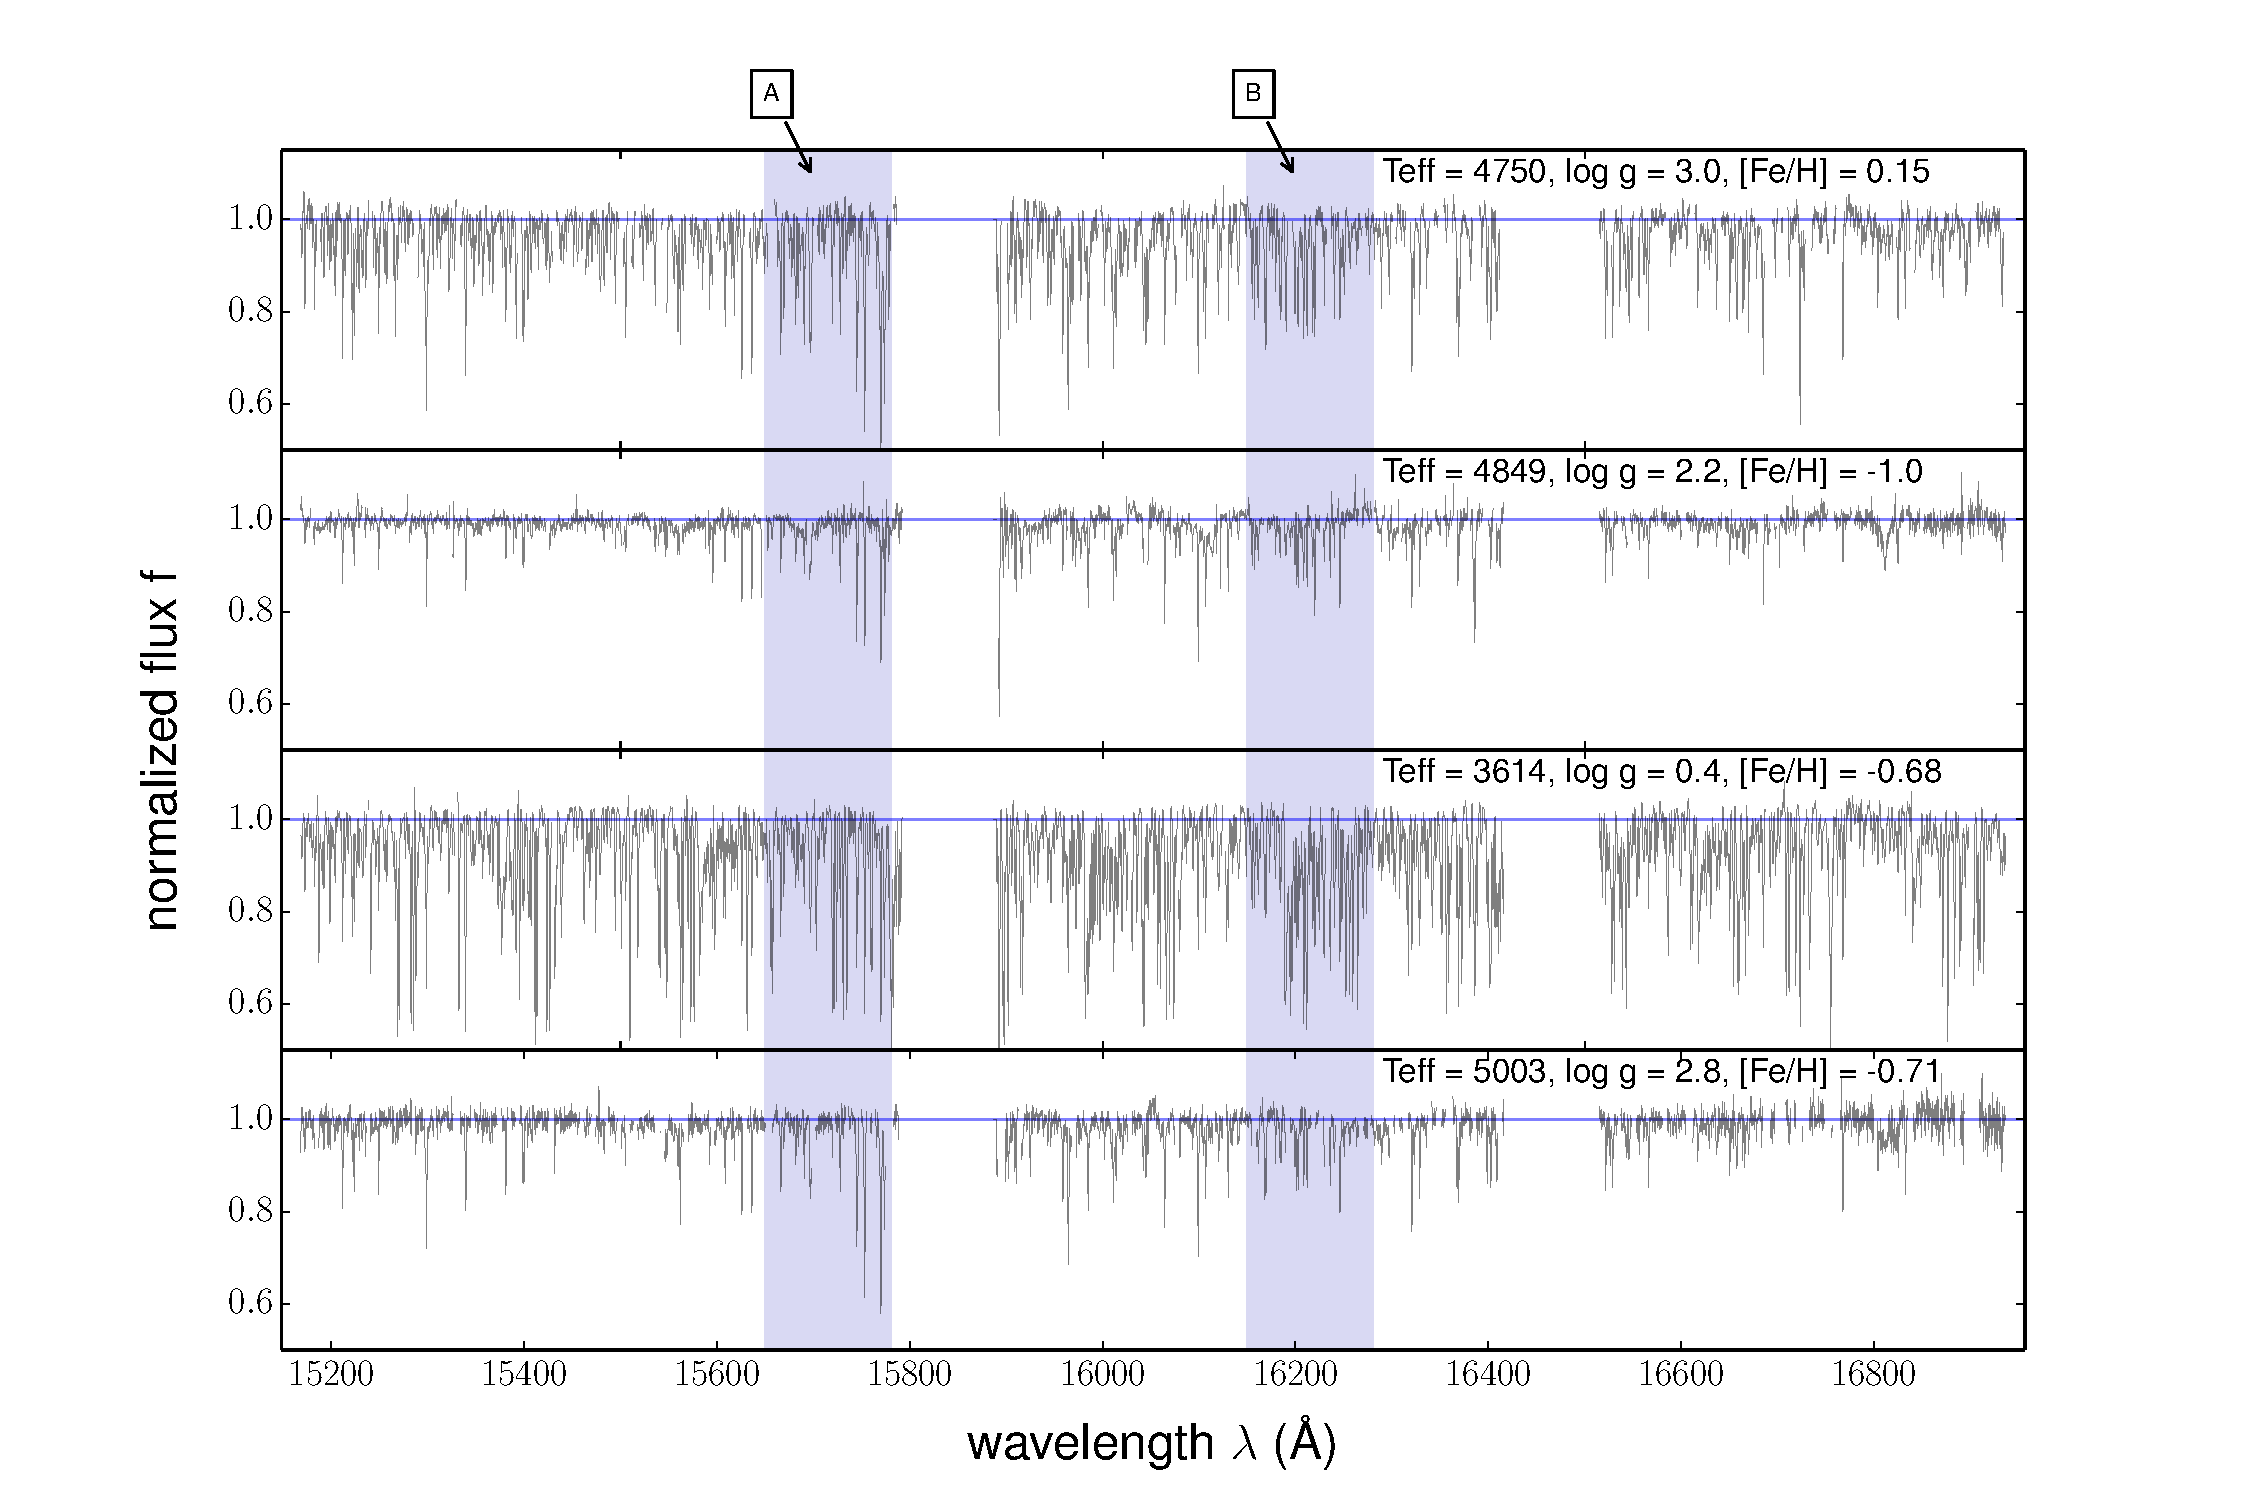
\includegraphics[height=\figureheight]{../documents/paper1/plots/four_examples3.pdf}
\end{frame}

\begin{frame}
  \frametitle{train, validate, and test}
  \begin{itemize}
  \item split the data into three disjoint subsets
  \item in the \emph{training step} you set the parameters of your model using the training set
  \item the validation set is used to set hyperparameters or model complexity
  \item in the \emph{test step} you apply the model to the test set---new data---to make predictions or deliver results
  \end{itemize}
\end{frame}

\begin{frame}
  \frametitle{\tc: Experiments}
  \begin{itemize}
  \item 1: train on cluster stars in \apogee, test on all of \apogee
    \begin{itemize}
    \item $\teff, \logg, \feh$
    \end{itemize}
  \item 2: train on \lamost--\apogee\ overlap, test on all of \lamost
    \begin{itemize}
    \item $\teff, \logg, \feh$
    \item label transfer
    \end{itemize}
  \item 3: train on asterosesimology--\apogee\ overlap, test on \apogee
    \begin{itemize}
    \item $\teff, \logg, \feh, \alphafe$, mass, age
    \end{itemize}
  \item 4: train on high-SNR \apogee, test on all of \apogee
    \begin{itemize}
    \item $\teff, \logg$, and 15 abundances
    \item de-noising
    \end{itemize}
  \end{itemize}
\end{frame}

\begin{frame}
  \frametitle{\tc\ experiment 1: training set}
  \begin{itemize}
  \item 543 stars (too few) from 19 clusters (too few)
  \item $\teff, \logg, \feh$ labels from \apogee
    \begin{itemize}
    \item calling parameters and abundances ``labels''
    \item slight adjustments to labels to get them onto possible isochrones
    \end{itemize}
  \item \emph{terrible} coverage of the main sequence
    \begin{itemize}
    \item only the Pleiades
    \item home-made Pleiades labels (by Ness)
    \item no $\feh$ spread at high $\logg$.
    \end{itemize}
  \end{itemize}
\end{frame}

\begin{frame}
  \frametitle{\tc\ experiment 1; training set}
  \,\hfill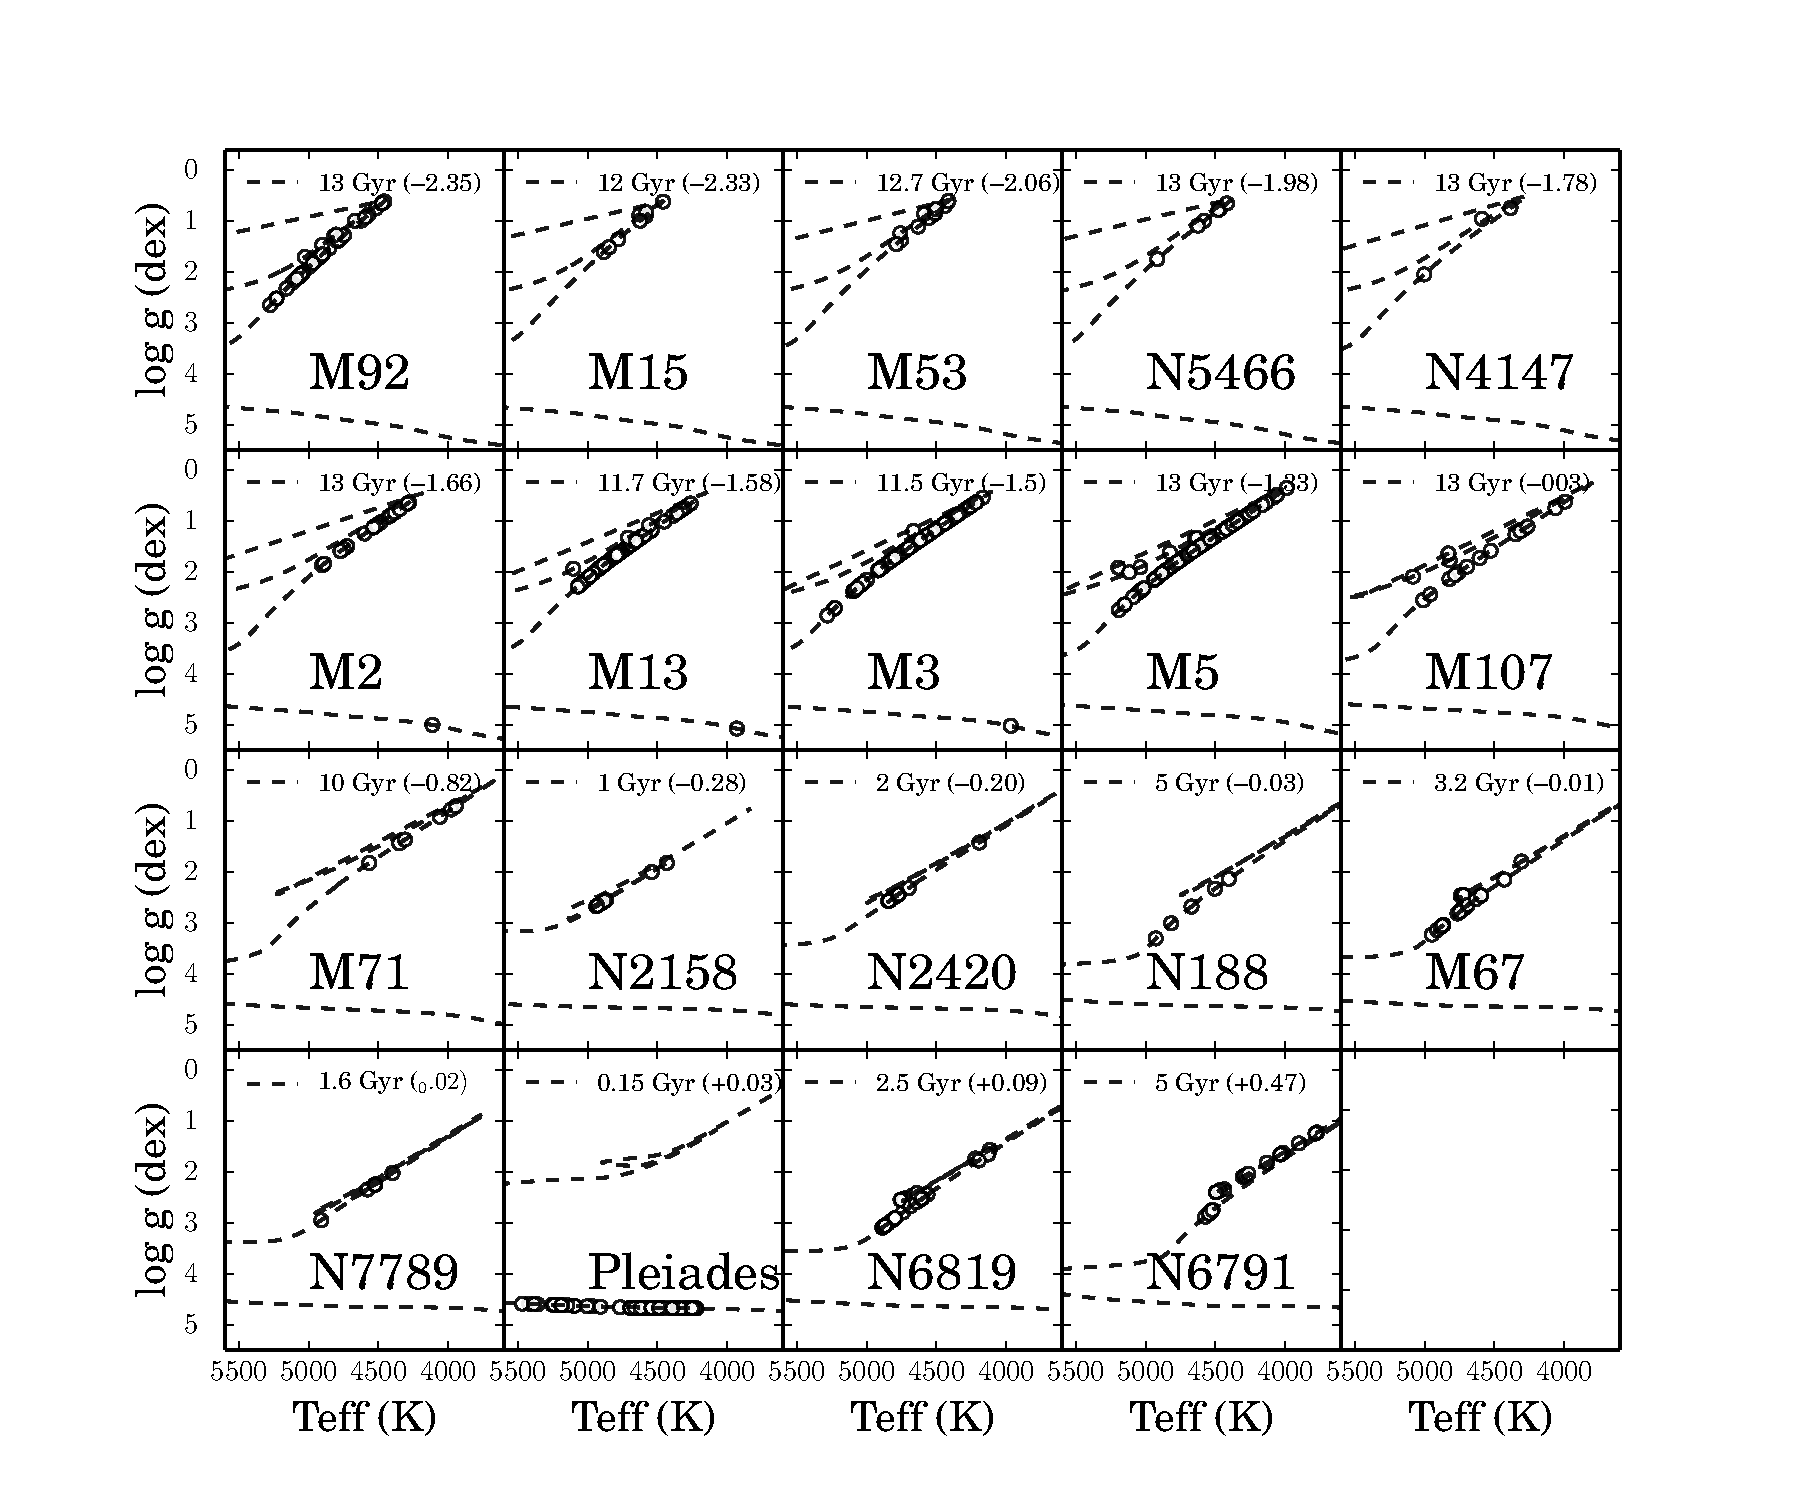
\includegraphics[height=\figureheight]{../documents/paper1/plots/training_mkn2.pdf}
\end{frame}

\newcommand{\flux}{f}
\newcommand{\fluxes}{\boldsymbol{\flux}}
\newcommand{\labels}{\boldsymbol{\ell}}
\newcommand{\pars}{\boldsymbol{\theta}}

\begin{frame}
  \frametitle{\tc: model}
  \begin{itemize}
  \item a \emph{generative model} of the \apogee\ spectra
    \begin{itemize}
    \item given label vector $\labels$, predict flux vector $\fluxes$
    \item probabilistic prediction $p(\fluxes\given\labels,\pars)$
    \end{itemize}
  \item use every spectral pixel's uncertainty variance $\sigma^2_{\lambda n}$ responsibly
  \item details:
    \begin{itemize}
    \item spectral expectation is quadratic in the labels
    \item every wavelength $\lambda$ treated independently
    \item an intrinsic Gaussian scatter $s^2_\lambda$ at every wavelength $\lambda$
    \item experiment 1: 80,000 free parameters in $\pars$!
    \item experiment 4: 1,400,000 free parameters!
    \end{itemize}
  \end{itemize}
\end{frame}

\begin{frame}
  \frametitle{\tc: model}
{\footnotesize
  \begin{eqnarray}
    \ln p(\fluxes_n\given\labels_n,\pars) &=& \sum_{\lambda=1}^L \ln p(\flux_{\lambda n}\given\labels_n,\pars_\lambda,s^2_\lambda)
    \nonumber \\
    \ln p(\flux_{\lambda n}\given\labels_n,\pars_\lambda,s^2_\lambda) &=& -\frac{1}{2}\,\frac{[f_{\lambda n} - \transpose{\pars_\lambda}\cdot\labels_n]^2}{\sigma^2_{\lambda n} + s^2_\lambda} + \ln (\sigma^2_{\lambda n} + s^2_\lambda)
    \nonumber \\
    \transpose{\labels} &\equiv& \left\{1, \teff, \logg, \feh,\right.
    \nonumber \\
                        & & \left.\teff^2, \teff\,\logg, \cdots, \feh^2\right\}
    \nonumber \\
    \transpose{\pars} &\equiv& \left\{\pars_\lambda, s^2_\lambda\right\}_{\lambda=1}^L
    \nonumber
  \end{eqnarray}
}
\end{frame}

\begin{frame}
  \frametitle{\tc: model}
  \begin{itemize}
  \item $\ln p(\fluxes_n\given\labels_n,\pars)$
  \item \emph{training step}: optimize w.r.t.\ parameters $\pars$ at fixed labels
    $\labels$ using training-set data
    \begin{itemize}
    \item linear least squares
    \item every wavelength $\lambda$ treated independently
    \end{itemize}
  \item \emph{test step}: optimize w.r.t.\ labels $\labels$ at fixed
    parameters $\pars$ using test-set (survey) data
    \begin{itemize}
    \item non-linear optimization
    \item every star treated independently
    \end{itemize}
  \end{itemize}
\end{frame}

\begin{frame}
  \frametitle{\tc\ experiment 1: training}
  \,\hfill\includegraphics<1>[width=\figurewidth]{./data_model_cyan.png}
\end{frame}

\begin{frame}
  \frametitle{\tc\ experiment 1: training}
  \,\hfill\includegraphics<1>[height=\figureheight]{../documents/paper1/plots/R1_continuum5.png}
\end{frame}

\begin{frame}
  \frametitle{\tc\ experiment 1: cross-validation}
  \,\hfill\includegraphics<1>[height=\figureheight]{../documents/paper1/plots/takeout_histc.png}
\end{frame}

\newcommand{\results}{%
\begin{frame}
  \frametitle{\tc\ experiment 1: results}
  \begin{itemize}
  \item \tc\ is far faster than physical modeling
    \begin{itemize}
    \item model trains in \emph{seconds} (thousands of fits)
    \item \tc\ labels $10^5$ stars per hour
    \item (pure Python on a laptop)
    \end{itemize}
  \item labels appear sensible
    \begin{itemize}
    \item \tc\ labels lie near sensible isochrones
    \item scatter against \apogee\ labels consistent with \apogee\ precision
    \end{itemize}
  \item successfully puts labels on dwarfs
  \end{itemize}
\end{frame}}

\results

\begin{frame}
  \frametitle{\tc\ experiment 1: comparison with \textsl{\acronym{ASPCAP}} labels}
  \,\hfill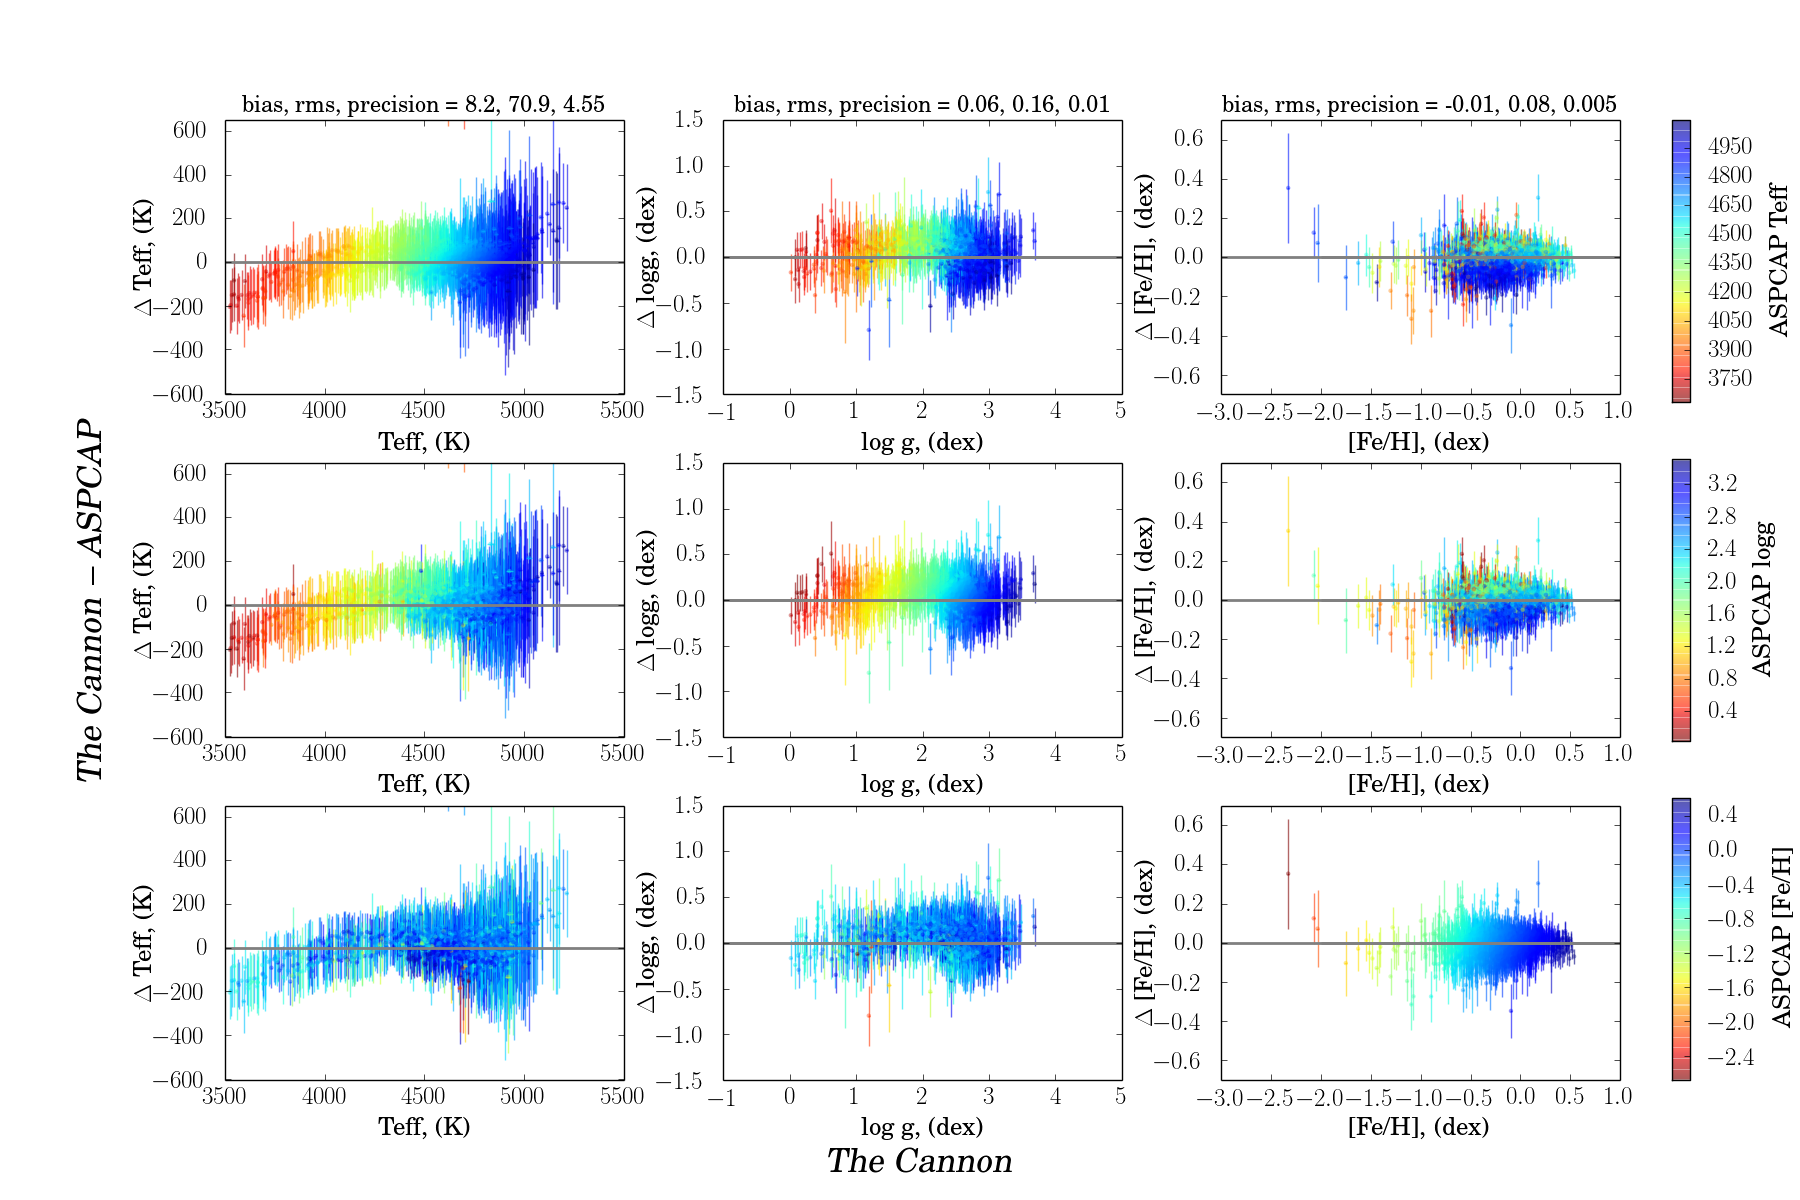
\includegraphics[height=\figureheight]{../documents/paper1/plots/cplot2.png} 
\end{frame}

\begin{frame}
  \frametitle{\tc\ experiment 1: label veracity}
  \,\hfill\includegraphics<1>[height=\figureheight]{../documents/paper1/plots/iso2_2.png}
         \includegraphics<2>[height=\figureheight]{../documents/paper1/plots/iso2a_2.png}
\end{frame}

\results

\begin{frame}
  \frametitle{\tc: shortcuts and choices}
  \begin{itemize}
  \item no Bayes; no partial or noisy labels
  \item quadratic order
    \begin{itemize}
    \item replacing polynomial with a Gaussian process
    \item continuous model complexity; non-parametric
    \end{itemize}
  \item spectral representation
  \item too-small training sets
  \end{itemize}
\end{frame}

\begin{frame}
  \frametitle{\tc\ experiment 3: masses and ages for red giants (Ness)}
  \,\hfill\includegraphics<1>[width=\figurewidth]{6labels_mass.png}%
          \includegraphics<2>[width=\figurewidth]{6labels_age.png}
\end{frame}

\begin{frame}
  \frametitle{\tc\ experiment 4: detailed abundances (Ness)}
  \,\hfill\includegraphics<1>[height=\figureheight]{../documents/abundances/20elem7_tc2_nofilt.png}%
          \includegraphics<2>[height=\figureheight]{../documents/abundances/20elem12_tc2_nofilt.png}%
          \includegraphics<3>[trim=0.5in 2in 0.5in 1.9in, width=\figurewidth]{sn.pdf}%
\end{frame}

\begin{frame}
  \frametitle{lessons learned}
  \begin{itemize}
  \item regressions are different from density estimators
  \item value of convex regularization
  \item de-noising
  \end{itemize}
\end{frame}

\begin{frame}
  \frametitle{\tc\ experiment 4: identification of lines (Casey)}
  \,\hfill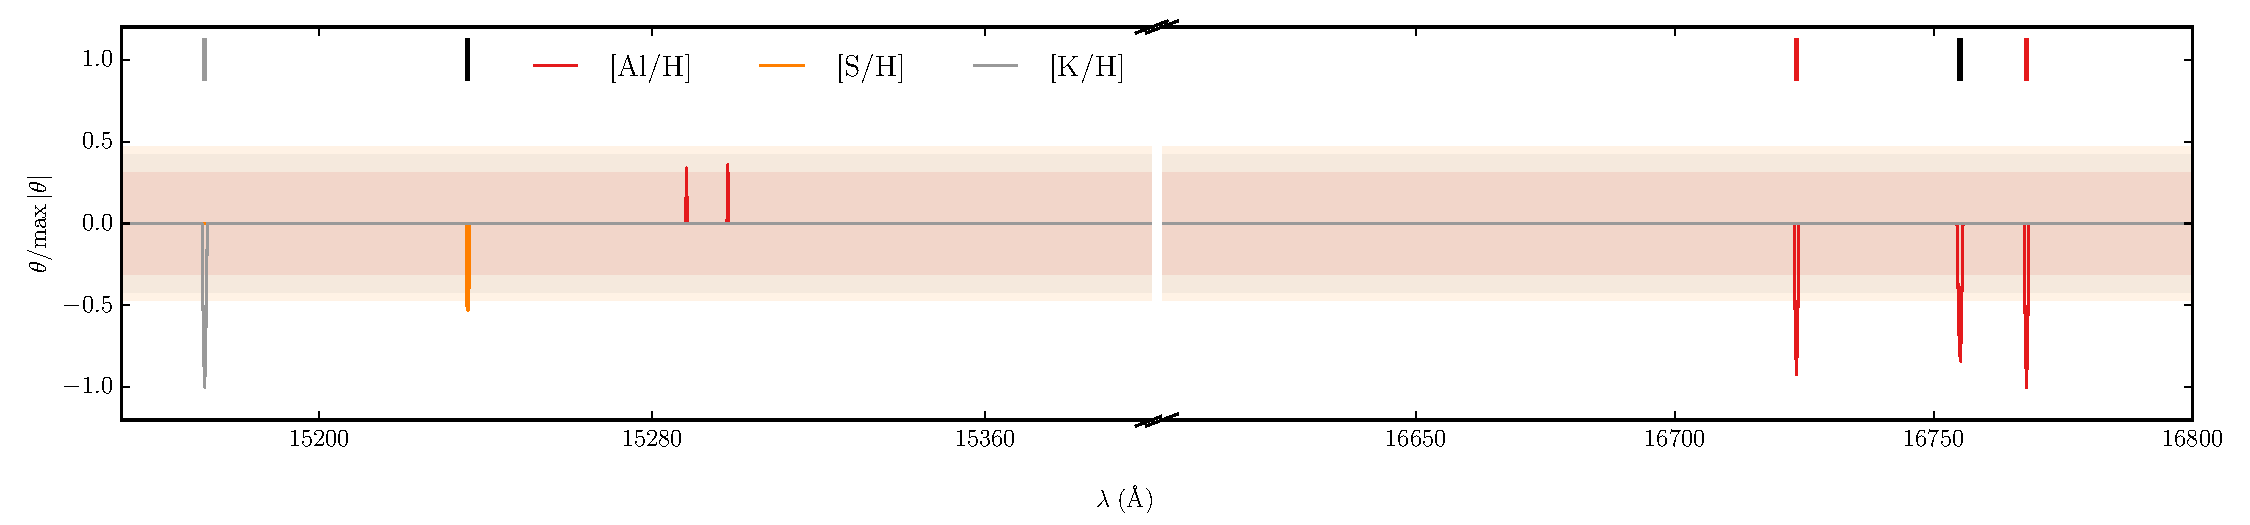
\includegraphics[width=\figurewidth]{sparse-first-order-coefficients.pdf}%
\end{frame}

\begin{frame}
  \frametitle{\tc\ experiment 2: discovery of outliers (Ho)}
  \,\hfill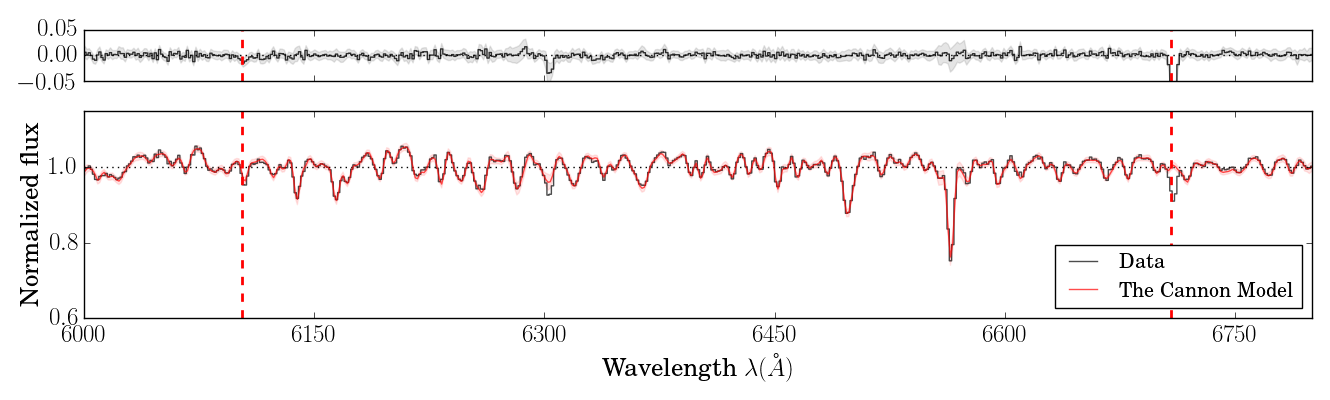
\includegraphics[width=\figurewidth]{resid_376.png}%
\end{frame}

\begin{frame}
  \frametitle{hierarchical models}
  \begin{itemize}
  \item every star has noisily observed data generated by its own (latent) parameters
  \item latent (true) parameters are drawn from distributions that are
    paraemeterized by hyper-parameters
  \item combine these into one big probabilistic model and fit everything simultaneously
  \end{itemize}
\end{frame}

\begin{frame}
  \frametitle{Self-calibration of the red clump (Hawkins)}
  \,\hfill\includegraphics<1>[height=\figureheight]{1705.08988/red_clump_pgm.pdf}
          \includegraphics<2>[height=\figureheight]{1705.08988/RCHRD_30per_tmass.pdf}
          \includegraphics<3>[height=\figureheight]{1705.08988/corner_Ks_final.pdf}
          \includegraphics<4>[height=\figureheight]{1705.08988/error_shrinkage_dist.pdf}
\end{frame}

\begin{frame}
  \frametitle{The full \tgas\ color-magnitude diagram (Anderson)}
  \,\hfill\includegraphics<1>[width=\figurewidth]{1706.05055/data.pdf}
          \includegraphics<2>[width=\figurewidth]{1706.05055/posteriorCMD.pdf}
          \includegraphics<3>[height=\figureheight]{1706.05055/posterior.pdf}
          \includegraphics<4>[height=\figureheight]{1706.05055/m67.pdf}
\end{frame}

\begin{frame}
  \frametitle{lessons learned}
  \begin{itemize}
  \item value of graphical models
  \item high-end MCMC samplers
    \begin{itemize}
    \item Don't use \project{emcee} when you have thousands to millions of parameters!
    \end{itemize}
  \item modeling outliers
  \end{itemize}
\end{frame}

\begin{frame}
  \frametitle{what I didn't say}
  \begin{itemize}
  \item How are we going to use these tools to measure the formation
    and dynamics of the Milky Way?
  \end{itemize}
\end{frame}

\begin{frame}
  \frametitle{read more}
  \begin{itemize}
  \item original paper on \tc\ and \apogee: Ness \etal\ arXiv:1501.07604
  \item labeling \lamost: Ho \etal\ arXiv:1602.00303
  \item labeling \project{\acronym{RAVE}}: Casey \etal\ arXiv:1609.02914
  \item chemical abundances: Casey \etal\ arXiv:1603.03040
  \item red-giant masses and ages: Ness \etal\ arXiv:1511.08204; Ho \etal\ arXiv:1609.03195
  \item homogeneity of clusters: Ness \etal\ arXiv:1701.07829
  \item chemical tagging: Hogg \etal\ arXiv:1601.05413
  \item calibrating the red clump: Hawkins \etal\ arXiv:1705.08988
  \item modeling the color-magnitude diagram: Leistedt \& Hogg arXiv:1703.08112; Anderson \etal\ arXiv:1706.05055
    \begin{itemize}
    \item \textsl{in prep}: working with missing and noisy labels
    \end{itemize}
  \end{itemize}
\end{frame}

\conclusions

\end{document}
